\begin{figure}[h]
    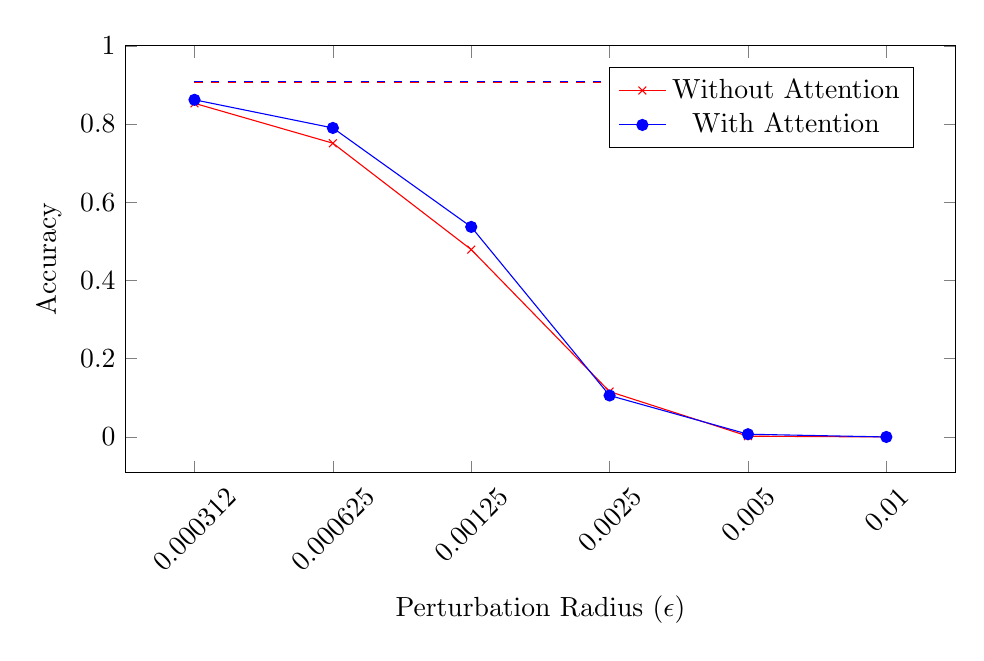
\begin{tikzpicture}
      \begin{axis}[xtick={0, 0.0003125, 0.000625, 0.00125, 0.0025, 0.005, 0.01}, x tick label style={rotate=45, log ticks with fixed point},xmode=log, log basis x=2, xlabel=Perturbation Radius ($\epsilon$), ylabel=Accuracy, width=\linewidth, height=7cm,legend style={at={(0.95,0.95)},anchor=north east}]
          
      \addplot[color=red,mark=x] coordinates {
        (0.0003125, 0.853)
        (0.000625, 0.751)
        (0.00125, 0.479)
        (0.0025, 0.116)
        (0.005, 0.002)
        (0.01, 0.0)
      };
      
      \addplot[color=blue,mark=*] coordinates {
        (0.0003125, 0.862)
        (0.000625, 0.790)
        (0.00125, 0.537)
        (0.0025, 0.106)
        (0.005, 0.007)
        (0.01, 0.0)
      };

      \addplot[color=red, domain=0.0003125:0.01, dashed]{0.906};
      \addplot[color=blue, domain=0.0003125:0.01, dashed]{0.909};
      
      \legend{Without Attention,With Attention}
      \end{axis}
      \end{tikzpicture}
    \caption{Clean- and robust-accuracy of InceptionResNetV2 models for skin lesion classification. Dashed lines represent clean-accuracy.}
    \label{IRV2DermRobustness}
  \end{figure}